\fancychapter{System Architecture}\label{chap:systemarch}
This chapter explains the full system architecture employed in this project. It will talk about all implementations, and the performance evaluation of each if possible. The focus will be on information:

Extracting information from unstructured data, using OCR engines and layout models.
Storing information with proper indexation for efficient semantic retrieval.
Employing prompt engineering techniques to enhance the consistency and accuracy of user interactions.

Building on the agentic approaches surveyed in Chapter~\ref{chap:stateofart}, we now present the concrete implementation of a semantic retrieval system that integrates these concepts into a practical architecture for enterprise document management.

\section{Optical Character Recognition (OCR)}\label{sec:ocr}
Most documents in this thesis were digitally born PDFs, from which text could be directly extracted using the \texttt{pdfreader} library. To ensure universal applicability of the \gls{RAG} pipeline, an \gls{OCR} fallback was implemented for cases where text was not embedded. 

OCR converts scanned PDFs or images into machine-readable text through preprocessing, segmentation, and recognition. Modern engines combine feature extraction, template matching, and contextual analysis using machine learning. Widely used options include Nougat \cite{blecher2023nougatneuralopticalunderstanding}, which preserves structure and outputs Markdown; Tesseract, an open-source tool supporting over 100 languages; and Google Vision API, a cloud-based service using deep neural networks for high accuracy.

In this thesis, Nougat is used because it is open-source and outputs Markdown, the preferred format for integration with large language models.

\section{Retrieval-Oriented Weaviate Schema in Edoclink}\label{sec:schema}

The first step involved defining a semantic data layer using Weaviate to capture the organizational logic of Edoclink documents. Six core classes were defined—Fluxo (workflow), Etapa (stage), Entidade (entity), Pasta (folder), Ficheiro (file), and Metadados (metadata)— which are connected via cross-references to enable traversal of organizational hierarchies while supporting semantic search and reasoning.

\begin{figure}[h!]
    \centering
    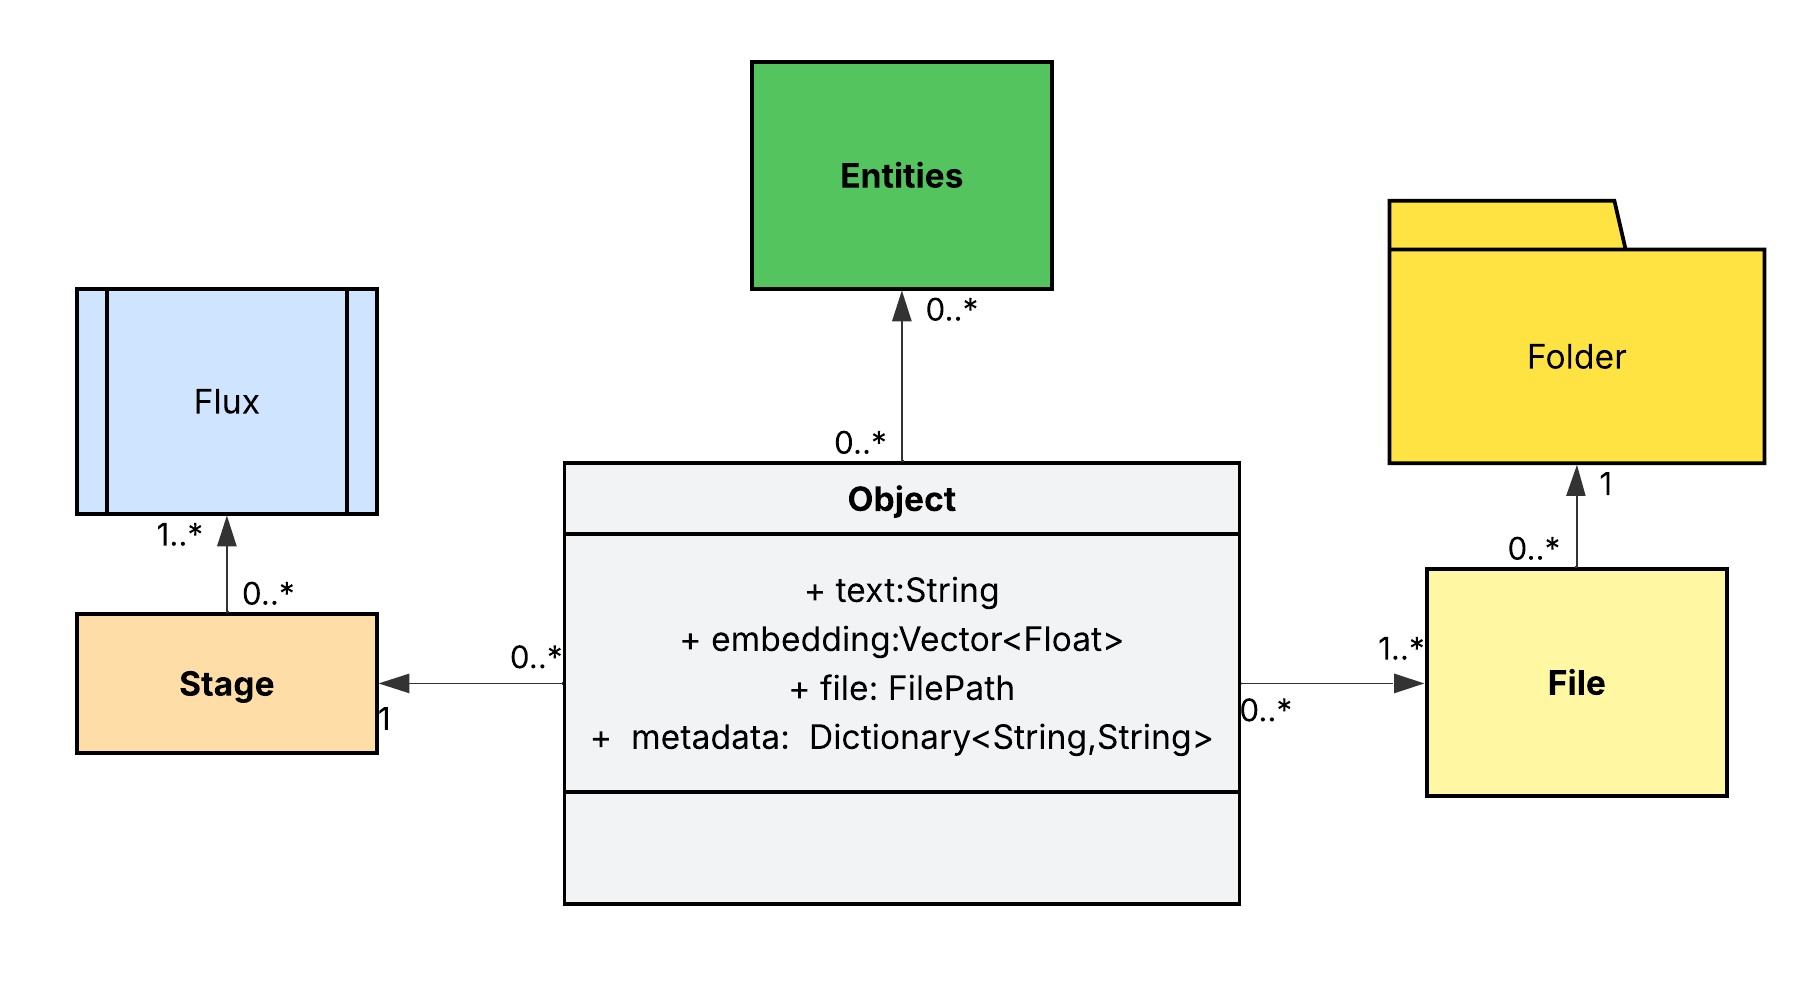
\includegraphics[width=1\linewidth]{Images/Classe UML.png}
    \caption{Abstract UML representation of a common corporate information schema, illustrating how documents, folders, and entities are typically organized and related within corporate repositories.}\label{fig:weaviate_class}
\end{figure}

The purpose for this research is to prove the possibility of semantic querying by organizational structure. A few examples were tested on a synthetically populated Weaviate database with this schema, including entities, stages, fluxes.

As research progressed, the schema evolved by embedding entity data, file paths, and metadata directly into object representations, enabling consistent deletion cascades and reducing reliance on cross-reference traversal. Figure~\ref{fig:weaviate_class} illustrates this abstract model, which served as a foundation for evaluating design choices. 
This diagram illustrates, the typical structure of how companies organizations organize their internal data. Most organizations adopt a hierarchical structure of \textbf{folders} and \textbf{files}, where documents are stored according to organizational preferences. In addition, many organizations structure their operations around projects, conceptualized as a \textbf{process flow}, comprising \textbf{stages}—such as development, production, or sales—typically arranged in sequential order.

As organizations scale, this structure becomes more complex, requiring higher-level abstractions. For example, companies may group information by \textbf{entities}, such as clients, suppliers, or internal employees, to track progress and associate multiple projects or files under each entity.


To leverage these structures for context-aware search and retrieval, it was used a\gls{AI} featured vector database, Weaviate, which is capable of managing multiple collections through a single instance. Each collection corresponds to one class defined in the UML model of Figure~\ref{fig:weaviate_class}, and cross-references were created between them. These cross-references represent the associations defined in the UML diagram, such as \textit{Fluxo--Etapa}, \textit{Entidade--Pasta}, and \textit{Pasta--Ficheiro}.

This implementation enables more structured semantic retrieval by allowing the system to traverse the logical hierarchy of the organization’s data during query execution. Rather than retrieving objects solely based on vector similarity, Weaviate can follow reference links to gather semantically related entities across collections. For example, a query about a specific project (\textit{Fluxo}) can automatically retrieve its corresponding \textit{Etapas}, or a search for an \textit{Entidade} can extend to all related \textit{Pastas} and their contained \textit{Ficheiros} and vice-versa.

By combining dense vector search with explicit relational connections, the system returns results that are semantically relevant and structurally consistent with corporate hierarchy. This design also enables structured traversal across corporate repositories—e.g., from an \textit{Entidade} to its \textit{Pastas} and their \textit{Ficheiros}, or from a \textit{Fluxo} to its \textit{Etapas}—which supports context-aware retrieval without inventing relationships or assumptions.

In practice, the real deployment is more complex, but this abstraction guided scalable semantic retrieval development for Edoclink.
Edoclink aims to store independent datasets under a shared schema, each exposed through webhooks that keep the database available and synchronized. Which can be easily done with Weaviate instances. This decentralized-style architecture distributes data across instances, increasing retrieval complexity because agents must identify and query appropriate webhooks when traversing datasets.

In summary, this section has focused on the database perspective: defining the schema and refining it through embedded fields, while keeping in mind decentralized scalable storage with efficient data distribution. The next section shifts attention to Agentic AI, where the challenge is not schema design but orchestrating retrieval with agents. This transition reflects the broader research landscape, where developments such as Weaviate's Query Agent \cite{weaviate} exemplify the move toward automated reasoning layers capable of multi-step retrieval and problem solving. 

\section{LLM-Based Metadata Extraction and Graph Construction}\label{sec:metadata_extraction}
The implemented system combines entity extraction, relationship identification, and graph-based storage to transform corporate documents into knowledge graphs. Documents are processed through a metadata extraction pipeline that integrates vector storage with graph-based knowledge representation, enabling search and reasoning over generated metadata rather than relying solely on lexical or semantic similarity.

The architecture is composed of two main pipelines:  
(1) Document ingestion and metadata extraction, and  
(2) Knowledge graph construction and querying.

\subsection{Document Ingestion and Metadata Extraction}

\begin{itemize}
    \item \textbf{Chunking:} Documents are segmented into overlapping text chunks through sentence tokenization, ensuring that each chunk contains full sentences with controlled overlap. This segmentation improves context preservation for downstream interactions.
    
    \item \textbf{Entity Extraction:} Using a \gls{LLM} guided by a few-shot prompt, the system identifies named entities within each chunk. Entities may represent \textit{projects, contracts, clients, departments, or financial elements}, depending on the examples and domain specificity of the few-shot configuration. Extracted entities are normalized and linked to their originating document.
    
    \item \textbf{Relationship Identification:} The system analyses co-occurrences and contextual dependencies among entities to infer semantic relationships. Relationships are derived from embedding-based proximity in the vector space.
    
    \item \textbf{Metadata Storage:} The resulting entities and relationships are stored across three complementary databases:
    \begin{itemize}
        \item a \textbf{Key-Value store} to hold raw document metadata (e.g., file path, document ID, author, date);
        \item a \textbf{Vector database} (e.g., Weaviate or NanoVector) to index embeddings of text chunks and entity descriptions;
        \item a \textbf{Knowledge graph} to capture structured relationships among entities and support relational reasoning.
    \end{itemize}
    This modular storage design allows both semantic retrieval and structured graph reasoning over the same dataset.
\end{itemize}
\begin{figure}
    \centering
    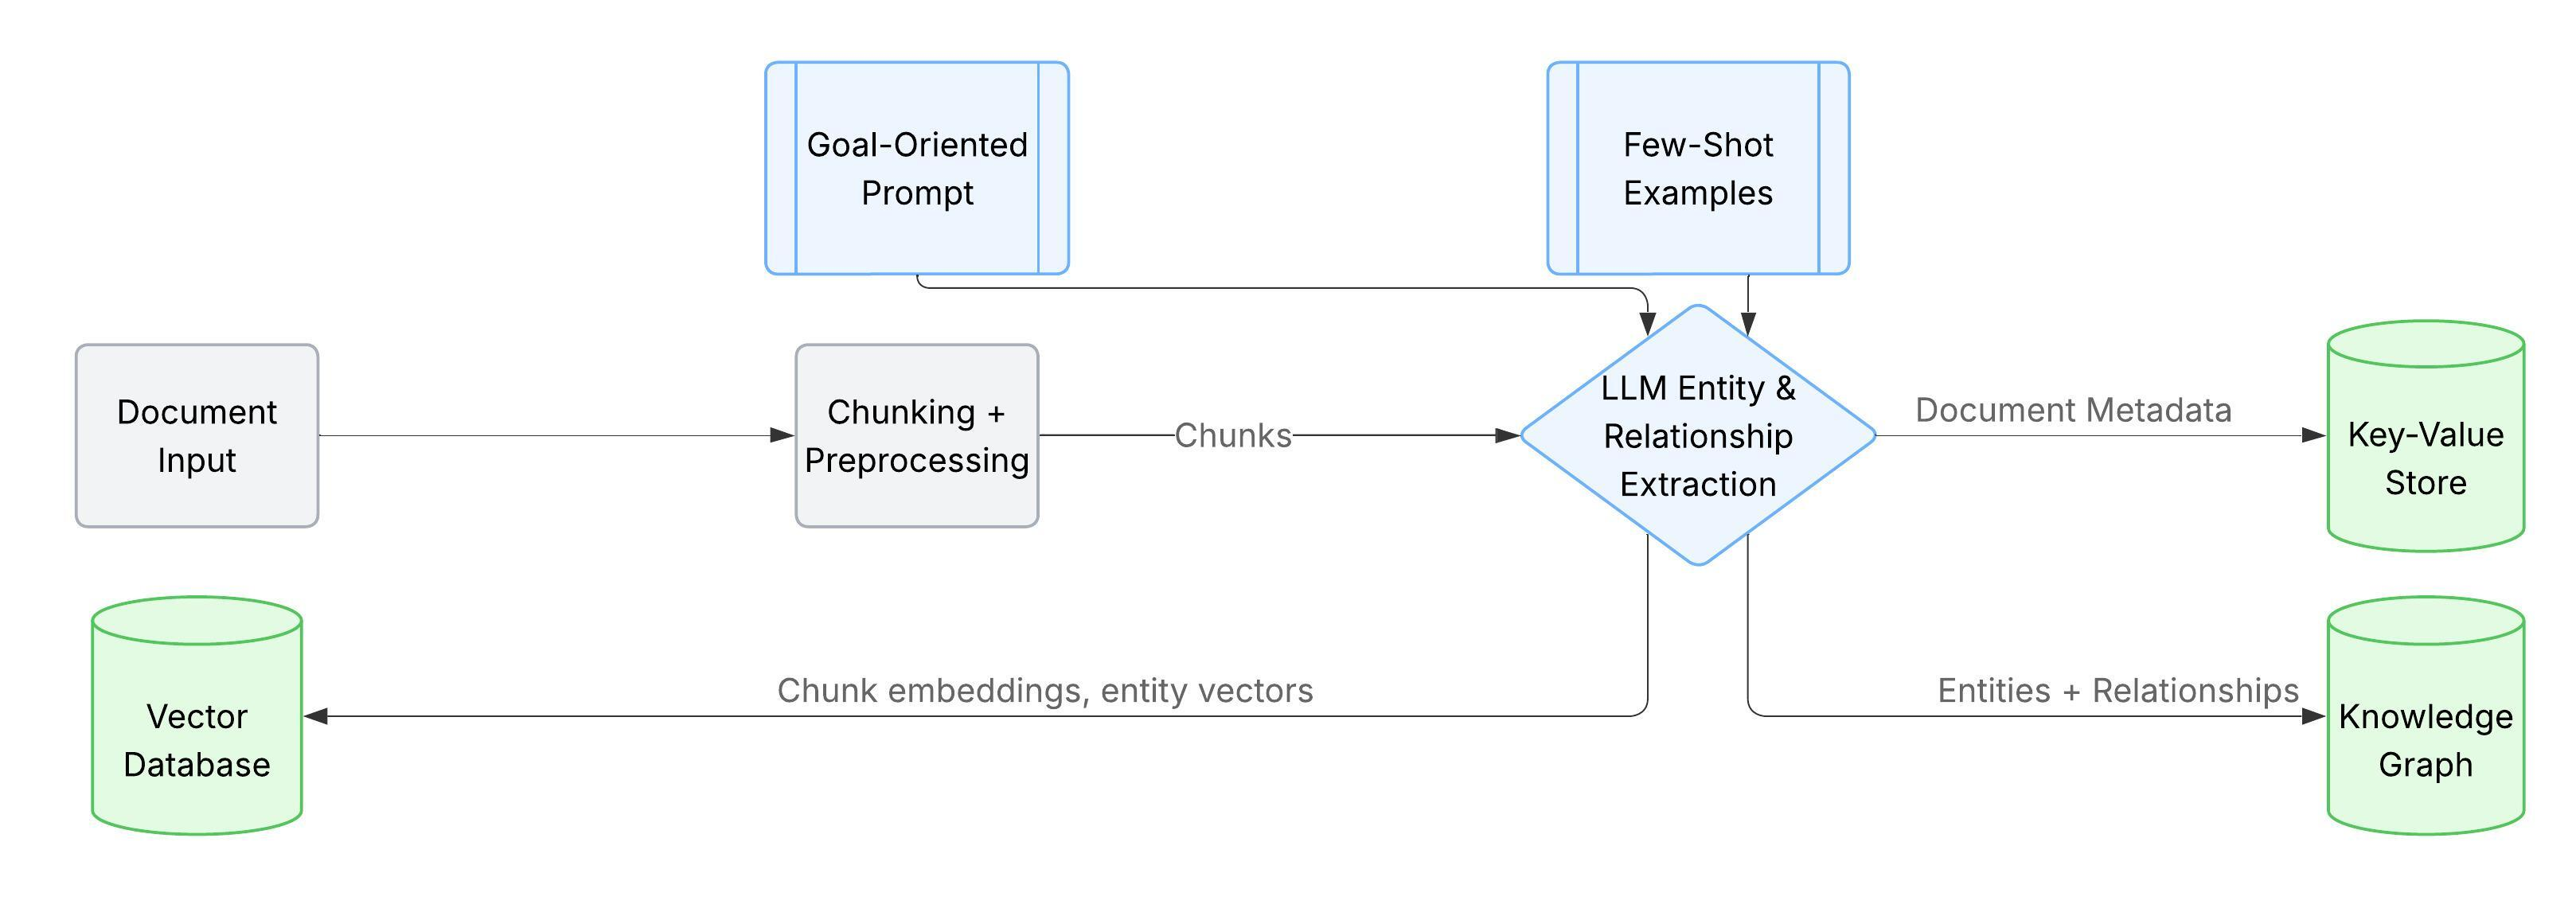
\includegraphics[width=1\linewidth]{Images/Fluxograma_Data_Processing_Pipeline.jpeg}
    \caption{Document Processing Pipeline.
Grey elements represent document preprocessing, blue elements denote LLM-driven information extraction, and green elements correspond to storage databases— vector, graph, and key–value}\label{fig:data-pipeline}
\end{figure}

\subsection{Knowledge Graph Construction}
The extracted metadata are organized into a heterogeneous graph that unifies textual, semantic, and relational information.

\begin{itemize}
    \item \textbf{Nodes} represent entities, document chunks, and other metadata fields.
    \item \textbf{Edges} represent relationships such as references, contextual links, or semantic similarity between entities.
\end{itemize}

The graph enables cross-document linking, allowing, for instance, all documents related  to the same project or supplier to be discovered through relational traversal.  
It also serves as a metadata index for future retrieval tasks or RAG-based agents, grounding responses in verifiable document sources.

\begin{figure}[H]
    \centering
    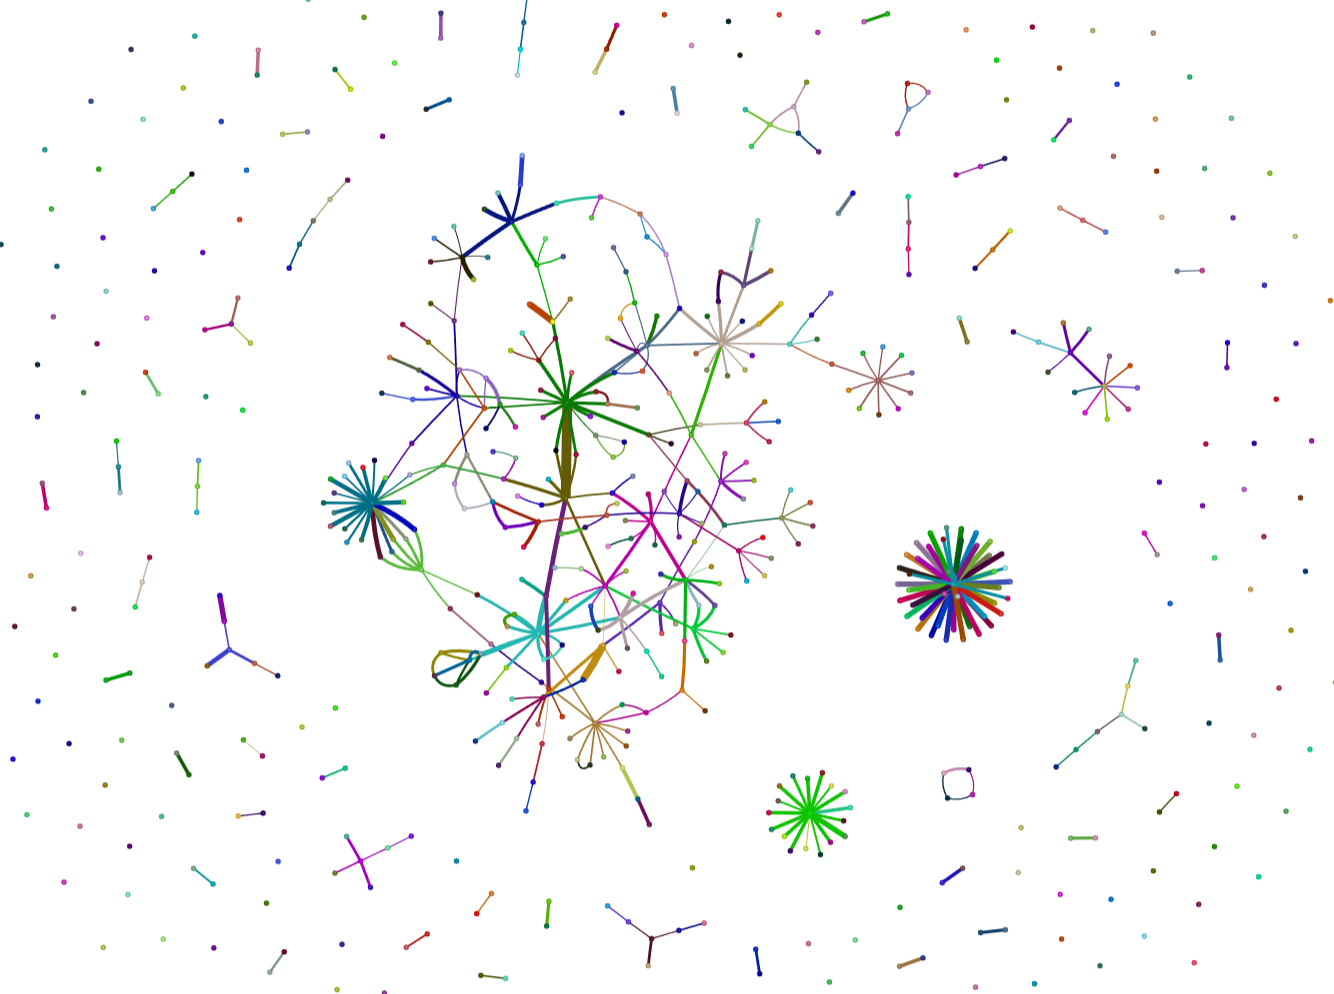
\includegraphics[width=0.5\linewidth]{Images/graph_visualisation_big.png}
    \caption{Knowledge graph from a thesis document about semantic retrieval}\label{fig:knowledge-graph}
\end{figure}

\subsection{Query Modes}

The system supports multiple query modes (\textit{mini}, \textit{light}, \textit{naive}, \textit{doc}, \textit{meta}, \textit{BM25}, and \textit{bypass}), each offering a different retrieval strategy:
\begin{itemize}
    \item \textbf{Mini} and \textbf{Light} modes use the knowledge graph to identify entities and relationships relevant to the query, enabling context-aware retrieval.
    \item \textbf{Naive} mode performs semantic search directly over entity embeddings stored in the vector database.
    \item \textbf{Doc} mode mirrors the naive retrieval but returns the list of relevant documents instead of generating a final answer.
    \item \textbf{Meta} mode performs keyword-based search over metadata fields, implemented with autocomplete support for strict metadata queries.
    \item \textbf{BM25} mode builds an index over all chunks and retrieves text via tokenised keyword matching.
\end{itemize}
\subsection{Mini Query Mode}

The \textit{Mini Query} mode performs multi-step reasoning over the knowledge graph to generate the most contextually accurate answer.  
It integrates keyword extraction, contextual retrieval, and answer generation within a single retrieval-augmented loop.

\begin{enumerate}
    \item \textbf{Keyword Extraction:}  
    An \gls{LLM} extracts answer-type keywords and entities from the user query using a predefined prompt (\texttt{PROMPTS["minirag\_query2kwd"]}).
    The extraction process is guided by the schema information available in the knowledge graph—specifically, the types and entities stored within it—to ensure semantic alignment between query terms and graph concepts.
    
    \item \textbf{Context Construction:}  
    Using the extracted entities and answer types, the system retrieves the corresponding nodes and relationships from the knowledge graph, along with matching embeddings from the \gls{VD}.
    These elements are then compiled into a structured context consisting of entity descriptions, related text chunks, and document snippets, forming the evidence base for the response.
    
    \item \textbf{Answer Generation:}  
    The compiled context is inserted into a response prompt (\texttt{PROMPTS["rag\_response"]}), and passed to the \gls{LLM}.
    The model synthesizes the final answer based on the retrieved contextual evidence, ensuring that generation remains grounded in verified document content.
\end{enumerate}

\begin{figure}
    \centering
    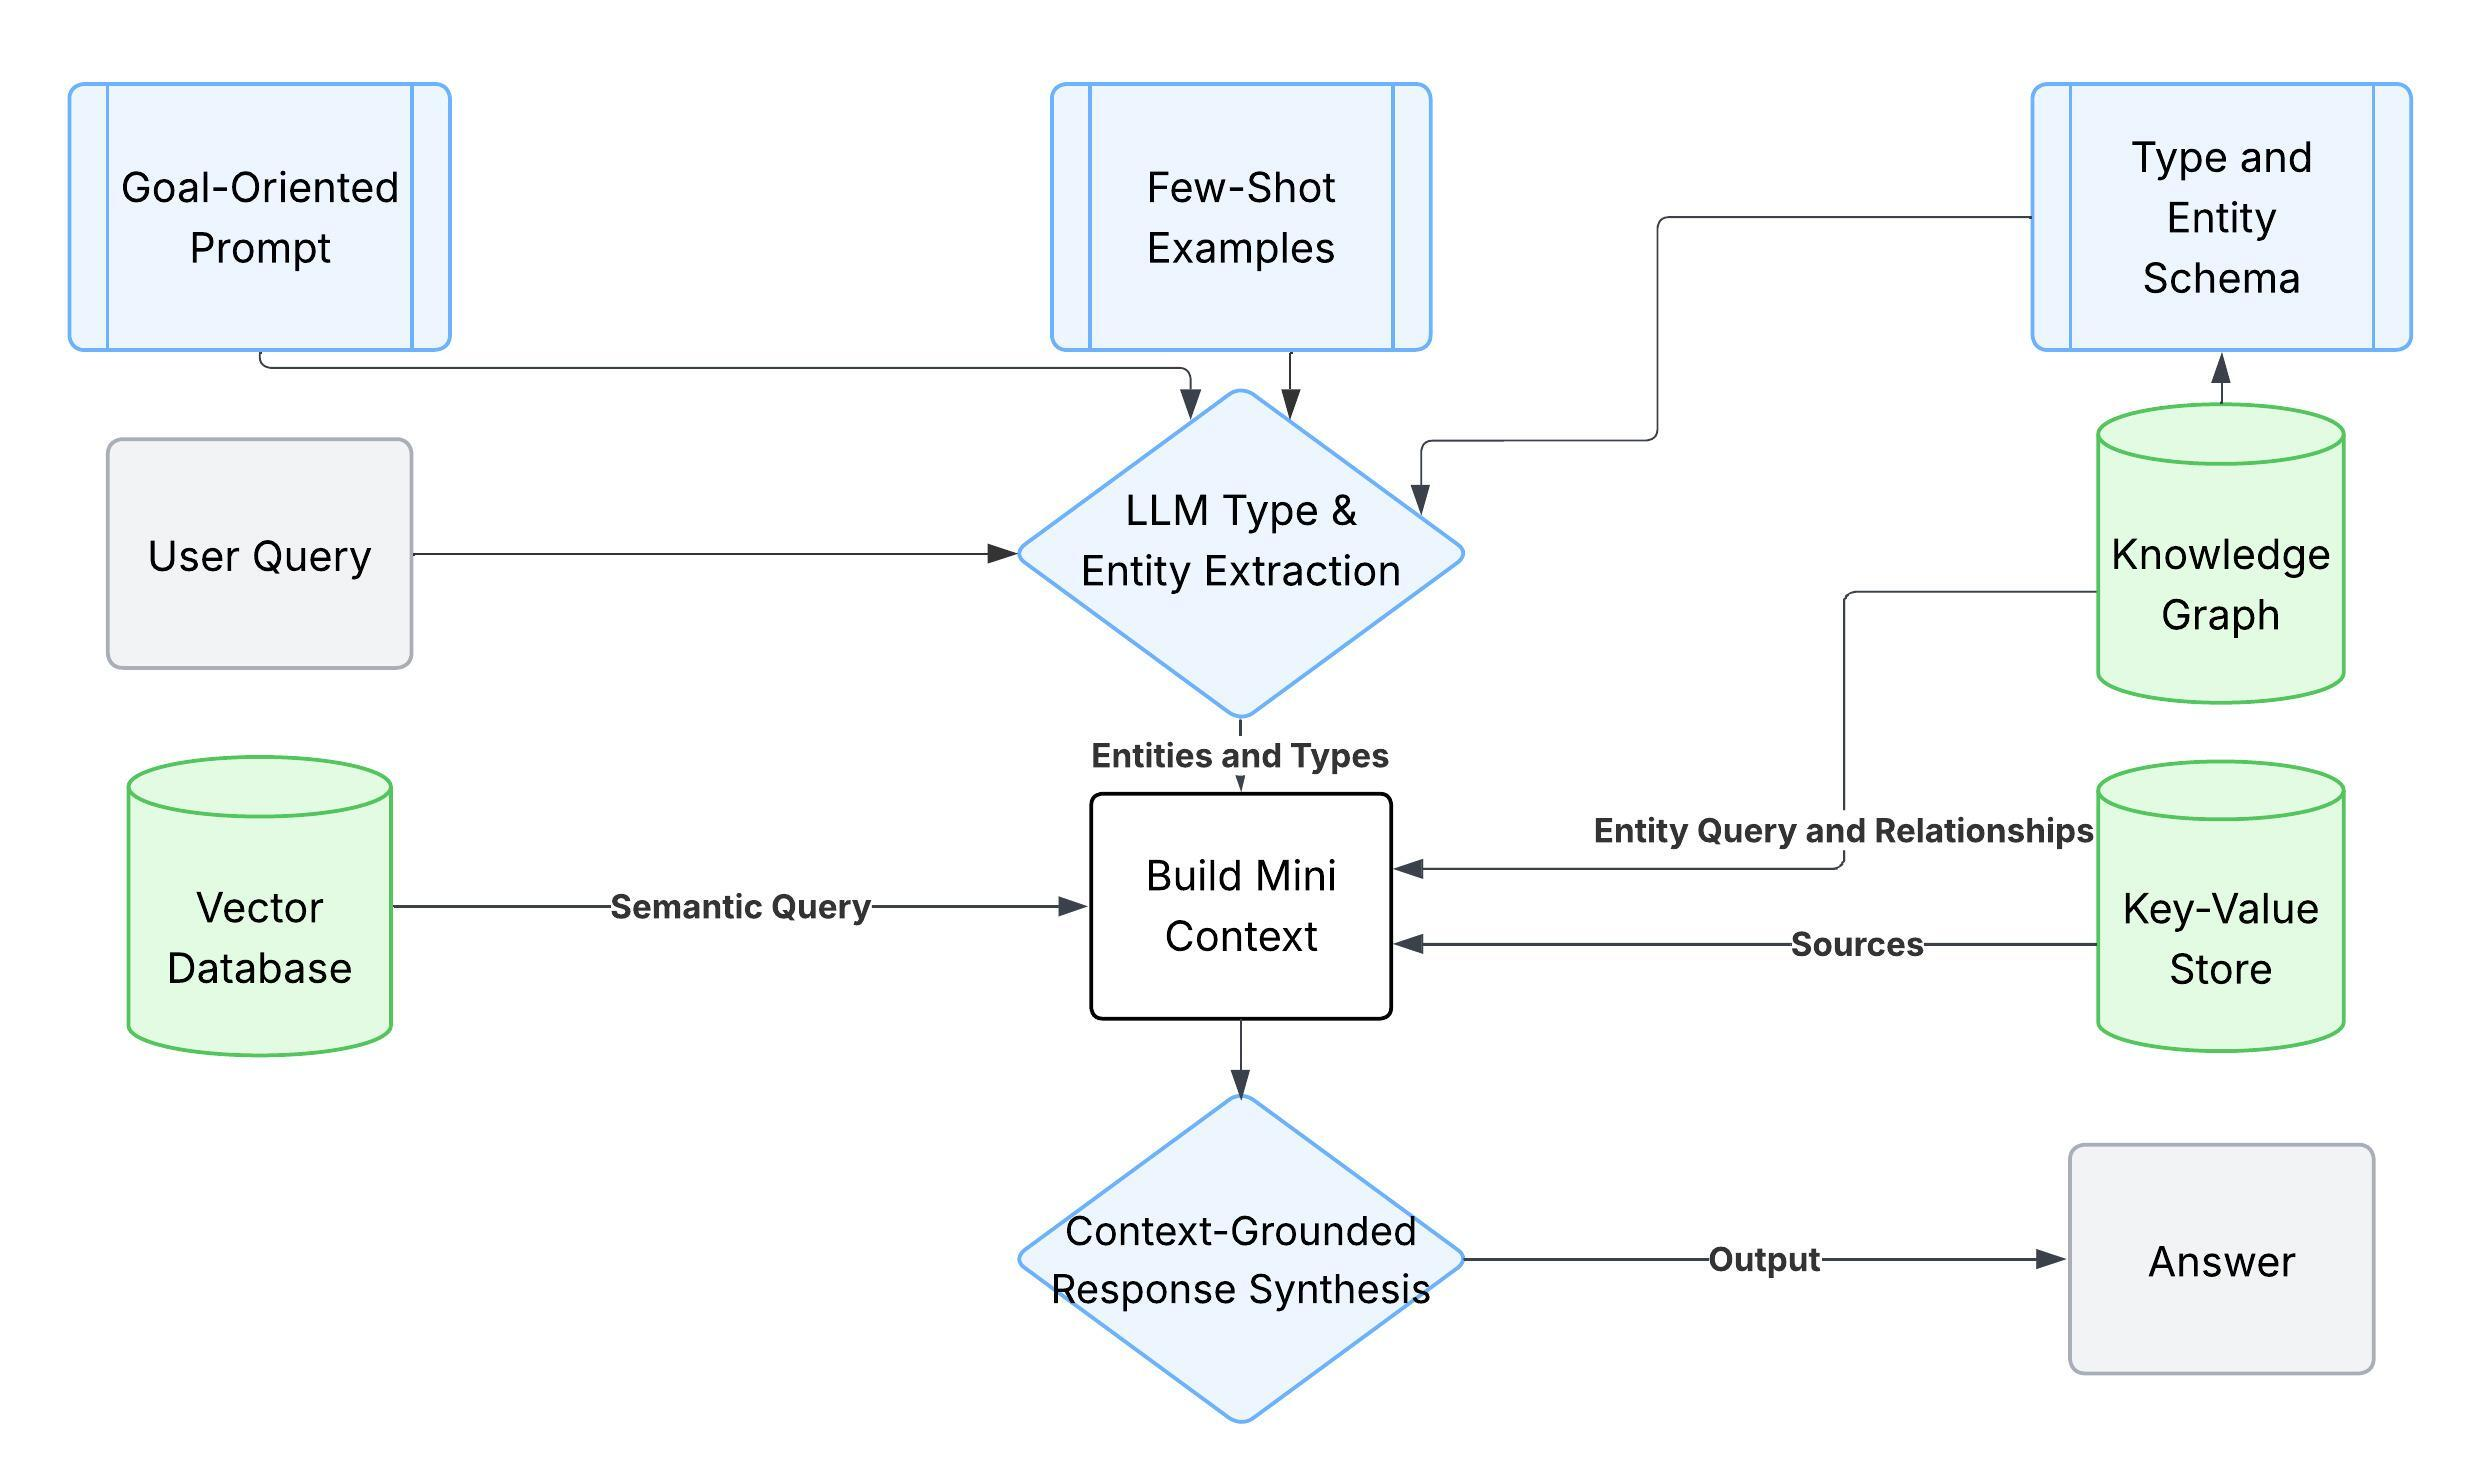
\includegraphics[width=0.75\linewidth]{Images/Fluxograma_Mini_Query.jpeg}
    \caption{Mini Query Flux}\label{fig:mini-query-flux}
\end{figure}

The diagram from Figure~\ref{fig:mini-query-flux} and subsequent diagrams follow ISO 5807 flowchart notation~\cite{iso5807}: rounded rectangles denote processes, diamonds represent decision or processing steps, cylinders indicate databases, and rectangles with double vertical edges signify predefined processes or constants.

\subsection{Weaviate Integration}

By leveraging MiniRAG's modular retrieval and storage design, a Weaviate integration was developed to enable automatic document insertion into the vector database following the defined schema, including automated cross-reference creation to mantain relational coherence. This architecture supports both retrieval and querying across cross-references, with documents automatically indexed according the organizational structure defined in Section~\ref{sec:schema}. The integration enables seamless flow from entity extraction and relationship identification directly into persistent storage, where the knowledge graph can later be queried and traversed by agents.

\subsection{Summary}

In summary, the implemented system transforms unstructured corporate documents into context-rich knowledge graphs by combining entity extraction, relationship identification, and graph-based storage. The Weaviate integration provides automatic indexing and cross-reference management, enriching the knowledge graph with explicit relational metadata. While these features were implemented and structurally validated, comprehensive benchmarking was limited by the absence of a properly formatted dataset capable of fully exercises the schema and cross-reference mechanisms. Nevertheless, the semantic layer provides a robust foundation for accurate information retrieval and supports graph-based visualization and exploration of meaningful relationships among documents, entities, and organizational processes.

\section{Weaviate MCP Server}\label{sec:weaviate-mcp-server}
A \glsxtrfull{MCP} server was developed to interface with a Weaviate vector database, with the primary goal of enabling interoperability. The MCP server enables clients such as \gls{LLM}-based agents to retrieve external information from Weaviate collections in a schema-aware manner. Since Weaviate databases typically enforce a strict schema, the server provides not only query tools but also maintains a memory of the available collections and their structure. This memory is extracted from the Weaviate schema endpoint and exposed to clients as MCP resources, thereby providing the agent with knowledge of valid properties before querying. When a client issues an invalid query, the server responds with an informative error listing the available fields, allowing the agent to self-correct its request automatically. The overall purpose of this server is to bridge information stored in Weaviate databases— with their dynamic, complex, and strict schemas— and powerful \gls{LLM} agents that reason over clients' requests and queries.

\subsection{Server Design}

The MCP server has been implemented in both Go and TypeScript. A Go implementation was necessary because the \texttt{mcp-registry} accepts pull requests only for Go servers. Moreover, Go offers excellent concurrency and produces lightweight binaries that are easy to containerize. If accepted, the Go version will be included in the official Docker registry, simplifying deployment.
%% Add here a diagram showing Go server

However, the project also provides a full TypeScript implementation. This version was refactored from the original Go codebase, with additional features enabled by the improved compatibility with both the Weaviate and Anthropic SDKs \cite{stainless_mcp_comparison}. While the Go version currently supports only \texttt{stdio} transport and hybrid querying, the TypeScript implementation extends functionality with HTTP transport and native Weaviate query generation using grouped tasks. These enhancements, along with stronger documentation and tighter integration with Weaviate's API, make the TypeScript version a more flexible and developer-friendly option, whereas Go remains easier to containerize, offering better compatibility with current \gls{MCP} registries.
%% Add here a diagram showing typescript Server
\subsection{Functionality}
The server functions as an intermediary between clients and the Weaviate backend. It registers the required tools and resources to support both querying and schema inspection. By exposing schema information as MCP resources (e.g., \texttt{weaviate://schema/Dataset}), the server enables clients to discover available collections, their properties (such as \texttt{targetProperties}: \{\texttt{text}: string, \texttt{filepath}: string\}) and cross-references (such as \texttt{refProperties} like \texttt{belongsToSomething} or \texttt{HasSomething}). This ensures that all interactions with the database are schema-aware and self-correcting, since invalid queries are met with descriptive feedback rather than failing silently (e.g., corrective validation logic shown in Figure~\ref{fig:sequence-diagram-weaviate-query}).
This design enables the use of Weaviate’s full toolkit, including object properties, multiple collections, and cross-references between them. Although ACL management is implemented within Edoclink, Weaviate natively supports this feature, which facilitates its use in secure and multi-tenant environments. Clients are typically \gls{LLM}-powered agents capable of communicating over \gls{MCP}, allowing them to seamlessly integrate external structured knowledge into their reasoning processes.

\subsection{MCP features}
The Weaviate MCP server exposes the following tools and resources to clients:
\begin{itemize}
    \item \textbf{\texttt{weaviate-query}}: Hybrid retrieval (vector + BM25) over a chosen collection. Inputs: \texttt{query}, \texttt{collection}, \texttt{targetProperties}, optional \texttt{limit} (default 3). Properties are validated against the collection schema; invalid fields yield a descriptive error listing valid ones. Returns the requested properties of the top-$k$ objects, with the vector signal prioritized over BM25.
    \item \textbf{\texttt{weaviate-generate-text}}: Same inputs as \texttt{weaviate-query}, but leverages Weaviate's generative grouped task to produce a concise answer grounded in the retrieved objects. Returns the generated text together with the structured result. This trades a small amount of latency---one additional LLM call---for a more concise response to the client.
    \item \textbf{\texttt{weaviate-origin}}: Collection-centric hybrid search that also summarizes first-hop cross-references (incoming and outgoing) discovered from the schema, and highlights unrequested ``missed'' fields. Helps plan the next traversal step by suggesting which references to follow.
    \item \textbf{\texttt{weaviate-follow-ref}}: One-hop traversal. Given a \texttt{collection}, a reference property \texttt{refProp}, base fields \texttt{baseProps}, referenced fields \texttt{refProps}, and optional \texttt{limit} (default 5), it runs a hybrid search and expands the chosen cross-reference, returning base objects with their referenced neighbors. All fields are validated against the base and target classes. This tool enables structured traversal across collections and implements cross-reference following as illustrated in Figure~\ref{fig:weaviate_class}. The implementation is dynamic: it discovers cross-references at inference time, enabling different collection schemas to be used without code changes.
    \item \emph{Schema resource}: In addition to tools, the server exposes collection schemas as MCP resources at \texttt{weaviate://schema/\{collection\}} so clients can discover available classes, properties, and references before querying.
\end{itemize}


\begin{figure}
    \centering
    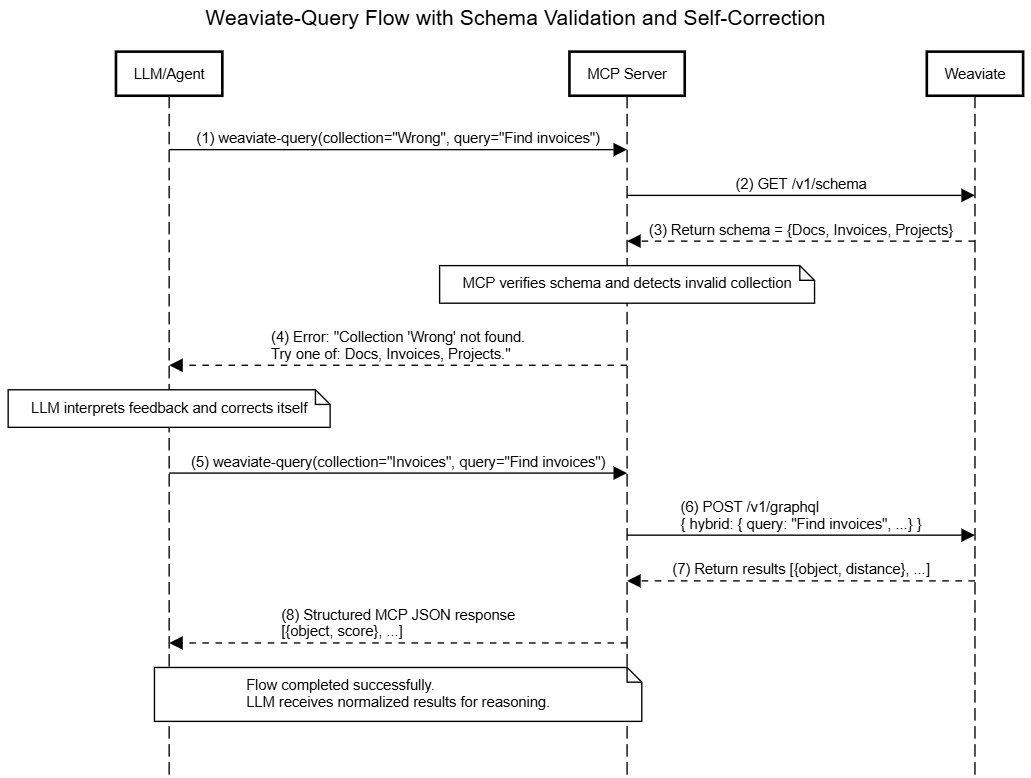
\includegraphics[width=1\linewidth]{Images/Sequence-diagram-Weaviate-Query.png}
    \caption{Sequence diagram of the \texttt{weaviate-query} tool illustrating the schema-aware approach used by the MCP Server to interface with an active Weaviate database. The same validation logic applies to other Weaviate schema elements that interface with the MCP Server.}\label{fig:sequence-diagram-weaviate-query}
\end{figure}

\section{System Limitations and Design Considerations}\label{sec:system-limitations}

While the proposed architecture provides a solid foundation for semantic search in enterprise environments, several limitations and design considerations should be noted:

\begin{itemize}
    \item \textbf{Scalability Constraints:} The current implementation uses HNSW indexing in Weaviate, which is efficient but requires storing all embeddings in memory. For very large-scale deployments (billions of documents), distributed vector databases using disk-based indexing might be necessary.
    
    \item \textbf{Embedding Quality:} The quality of semantic retrieval is directly dependent on the embedding model used. While \textit{all-MiniLM-L6-v2} provides good performance, domain-specific embedding models trained on enterprise corpora may yield better results.
    
    \item \textbf{Hallucination in LLMs:} Even when using \gls{RAG}, large language models may hallucinate or produce plausible-sounding yet incorrect information. The grounding in retrieved documents mitigates but does not eliminate this risk.
    
    \item \textbf{Privacy and Security:} Embeddings and retrieved documents are processed in external APIs (e.g., OpenAI). For highly sensitive data, on-premises \gls{LLM} deployments may be required, though this comes at the expense of reduced performance.
    
    \item \textbf{Cost at Scale:} While \gls{GPT}-4o offers superior reasoning, its cost scales with the number of queries. Cost-conscious deployments may need to balance accuracy against budget constraints using smaller models.
    
    \item \textbf{Knowledge Graph Completeness:} The automated knowledge graph construction is limited by the quality of entity extraction and relationship inference. Manual curation or domain-specific training can improve coverage.
    
    \item \textbf{Metadata Quality:} The system's effectiveness depends on consistent, high-quality metadata. Heterogeneous or poorly maintained metadata repositories may degrade retrieval performance.
    
\end{itemize}

These limitations are addressed partly through experimental validation (Chapter~\ref{chap:results}) and provide direction for future work (Chapter~\ref{chap:conclusion}).





